
%\definecolor{ublue}{rgb}{0.152,0.250,0.545}
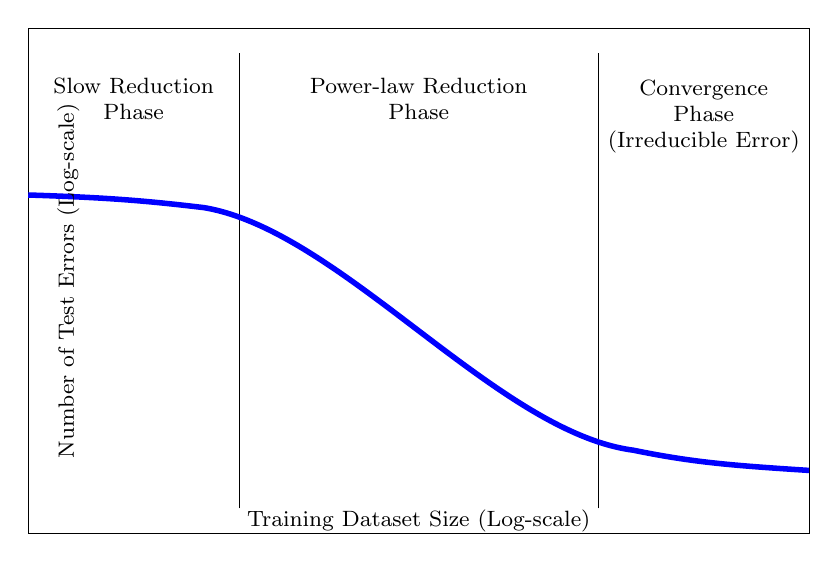
\begin{tikzpicture}

\def\upline{13.5}
\def\downline{2.5}
\def\upcenpos{17.2}

\begin{scope}
\begin{axis}[
width=11.5cm, height=8cm,
%symbolic x coords={1-15,16-25,26-35,>35},
%ytick={0,4,8,...,20},
%xtick={0,5,...,100},
xlabel={Training Dataset Size (Log-scale)},
ylabel={Number of Test Errors (Log-scale)},
xlabel style={align=center,yshift=1.2em,font=\footnotesize},
ylabel style={align=center,yshift=-2.2em,font=\footnotesize},
xticklabel style={fill=white,opacity=0},
yticklabel style={fill=white,opacity=0},
x tick style={fill=white,opacity=0},
y tick style={fill=white,opacity=0},
xtick=\empty,
ytick=\empty,
%x tick label style={font=\footnotesize},
%y tick label style={font=\footnotesize},
%tick align=inside,
%major grid style={draw=blue,dashed},
legend pos=outer north east,
%legend style={anchor=north west,yshift=-1cm},
%legend style={yshift=-4.5em,xshift=-6em,legend cell align=left,legend plot pos=right},
xmin=0,
xmax=100,
ymin=0,
ymax=20]
%\addplot [sharp plot,thick,blue] coordinates{(3,\upline) (22.5,13) (77.5, 3) (97, \downline)};

%\addplot [sharp plot,thick,blue,domain=2:23] (x,-0.00099*x*x+\upline-0.1);
%\addplot [sharp plot,thick,blue,domain=23:77] (x,-0.18*x+17.05);
%\addplot [sharp plot,thick,blue,domain=77:97] (x,0.001475*x^2 - 0.28615*x+13.878275+\downline+0.1);

\addplot [sharp plot] coordinates{(27,1) (27,19)};
\addplot [sharp plot] coordinates{(73,1) (73,19)};

%\addplot [sharp plot,very thick,dashed,green] coordinates{(2,\upline) (98,\upline)};
%\addplot [sharp plot,very thick,dashed,red] coordinates{(2,\downline) (98,\downline)};
{\footnotesize
\node[anchor=center,align=center,font=\footnotesize] (t1) at (axis cs:13.5,\upcenpos) {Slow Reduction\\ Phase};
\node[anchor=center,align=center,font=\footnotesize] (t2) at (axis cs:50,\upcenpos){Power-law Reduction\\ Phase};
\node[anchor=center, align=center,font=\footnotesize] (t3) at (axis cs:86.5,\upcenpos - 0.7) {Convergence \\ Phase \\ (Irreducible Error)};


%\draw[-,thick,purple] (axis cs:0,\upline-0.1) .. controls ([xshift=0em,yshift=0em]axis cs:0,\upline) and ([xshift=0em,yshift=-1em]axis cs:0,\upline) .. (axis cs:22.5,\upline-0.6);
\draw[-,line width=2pt,blue] (axis cs:0,\upline-0.1) .. controls ([xshift=0em,yshift=0em]axis cs:10,\upline-0.199) and ([xshift=0em,yshift=0em]axis cs:15,\upline-0.32275) .. (axis cs:22.5,\upline-0.6) .. controls ([xshift=0em,yshift=0em]axis cs:40,12) and ([xshift=0em,yshift=0em]axis cs:60,4) .. (axis cs:77.5,\downline+0.8) .. controls ([xshift=0em,yshift=0em]axis cs:85,\downline+0.32275) and ([xshift=0em,yshift=0em]axis cs:90,\downline+0.199) .. (axis cs:100,\downline);
}
%\addplot [sharp plot,very thick,orange,mark=*] coordinates{(1-15,17.5) (16-25,24) (26-35,25) (>35,27)};
%\legend{\tiny{NMT},\tiny{SPB},\tiny{HPB},\tiny{PBSY}}
\end{axis}
\end{scope}
\end{tikzpicture}

%---------------------------------------------------------------------
